\section{Model3DRigid  Class Reference}
\label{classModel3DRigid}\index{Model3DRigid@{Model3DRigid}}
A rigid robot in a 3D world. 


{\tt \#include $<$model3d.h$>$}

Inheritance diagram for Model3DRigid::\begin{figure}[H]
\begin{center}
\leavevmode
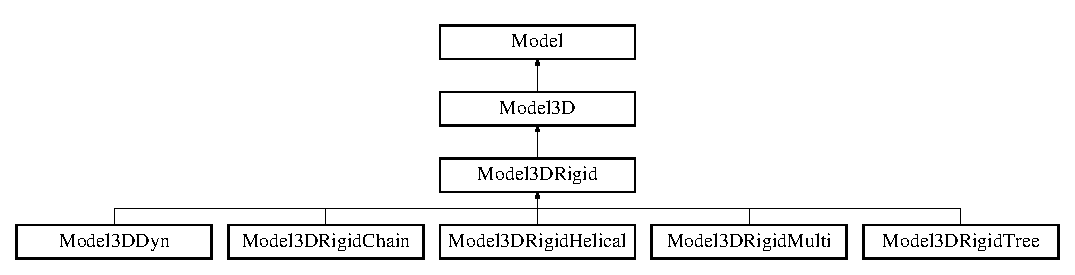
\includegraphics[height=3.24638cm]{classModel3DRigid}
\end{center}
\end{figure}
\subsection*{Public Methods}
\begin{CompactItemize}
\item 
{\bf Model3DRigid} (string path)
\item 
virtual {\bf $\sim$Model3DRigid} ()
\item 
virtual {\bf MSLVector} {\bf Integrate} (const {\bf MSLVector} \&x, const {\bf MSLVector} \&u, const double \&h)
\begin{CompactList}\small\item\em Perform integration from state x, using input u, over time step h.\item\end{CompactList}\item 
{\bf MSLVector} {\bf State\-Transition\-Equation} (const {\bf MSLVector} \&x, const {\bf MSLVector} \&u)
\begin{CompactList}\small\item\em The state transition equation, or equations of motion, xdot=f(x,u).\item\end{CompactList}\item 
virtual double {\bf Metric} (const {\bf MSLVector} \&x1, const {\bf MSLVector} \&x2)
\begin{CompactList}\small\item\em A distance metric, which is Euclidean in the base class.\item\end{CompactList}\item 
virtual {\bf MSLVector} {\bf Linear\-Interpolate} (const {\bf MSLVector} \&x1, const {\bf MSLVector} \&x2, const double \&a)
\begin{CompactList}\small\item\em Linearly interpolate two state while respecting topology.\item\end{CompactList}\end{CompactItemize}


\subsection{Detailed Description}
A rigid robot in a 3D world.



\subsection{Constructor \& Destructor Documentation}
\index{Model3DRigid@{Model3DRigid}!Model3DRigid@{Model3DRigid}}
\index{Model3DRigid@{Model3DRigid}!Model3DRigid@{Model3DRigid}}
\subsubsection{\setlength{\rightskip}{0pt plus 5cm}Model3DRigid::Model3DRigid (string {\em path} = \char`\"{}\char`\"{})}\label{classModel3DRigid_a0}


\index{Model3DRigid@{Model3DRigid}!~Model3DRigid@{$\sim$Model3DRigid}}
\index{~Model3DRigid@{$\sim$Model3DRigid}!Model3DRigid@{Model3DRigid}}
\subsubsection{\setlength{\rightskip}{0pt plus 5cm}Model3DRigid::$\sim$Model3DRigid ()\hspace{0.3cm}{\tt  [inline, virtual]}}\label{classModel3DRigid_a1}




\subsection{Member Function Documentation}
\index{Model3DRigid@{Model3DRigid}!Integrate@{Integrate}}
\index{Integrate@{Integrate}!Model3DRigid@{Model3DRigid}}
\subsubsection{\setlength{\rightskip}{0pt plus 5cm}{\bf MSLVector} Model3DRigid::Integrate (const {\bf MSLVector} \& {\em x}, const {\bf MSLVector} \& {\em u}, const double \& {\em h})\hspace{0.3cm}{\tt  [virtual]}}\label{classModel3DRigid_a2}


Perform integration from state x, using input u, over time step h.



Reimplemented from {\bf Model} {\rm (p.\,\pageref{classModel_a5})}.

Reimplemented in {\bf Model3DRigid\-Helical} {\rm (p.\,\pageref{classModel3DRigidHelical_a3})}.\index{Model3DRigid@{Model3DRigid}!LinearInterpolate@{LinearInterpolate}}
\index{LinearInterpolate@{LinearInterpolate}!Model3DRigid@{Model3DRigid}}
\subsubsection{\setlength{\rightskip}{0pt plus 5cm}{\bf MSLVector} Model3DRigid::Linear\-Interpolate (const {\bf MSLVector} \& {\em x1}, const {\bf MSLVector} \& {\em x2}, const double \& {\em a})\hspace{0.3cm}{\tt  [virtual]}}\label{classModel3DRigid_a5}


Linearly interpolate two state while respecting topology.

If a=0, then x1 is returned; if a=1, then x2 is returned. All intermediate values of \$a $\backslash$in [0,1]\$ yield intermediate states. This method is defined by {\bf Model} {\rm (p.\,\pageref{classModel})}. 

Reimplemented from {\bf Model} {\rm (p.\,\pageref{classModel_a6})}.

Reimplemented in {\bf Model3DRigid\-Multi} {\rm (p.\,\pageref{classModel3DRigidMulti_a3})}, {\bf Model3DRigid\-Chain} {\rm (p.\,\pageref{classModel3DRigidChain_a4})}, and {\bf Model3DRigid\-Tree} {\rm (p.\,\pageref{classModel3DRigidTree_a4})}.\index{Model3DRigid@{Model3DRigid}!Metric@{Metric}}
\index{Metric@{Metric}!Model3DRigid@{Model3DRigid}}
\subsubsection{\setlength{\rightskip}{0pt plus 5cm}double Model3DRigid::Metric (const {\bf MSLVector} \& {\em x1}, const {\bf MSLVector} \& {\em x2})\hspace{0.3cm}{\tt  [virtual]}}\label{classModel3DRigid_a4}


A distance metric, which is Euclidean in the base class.



Reimplemented from {\bf Model} {\rm (p.\,\pageref{classModel_a9})}.

Reimplemented in {\bf Model3DRigid\-Multi} {\rm (p.\,\pageref{classModel3DRigidMulti_a2})}, {\bf Model3DRigid\-Chain} {\rm (p.\,\pageref{classModel3DRigidChain_a5})}, and {\bf Model3DRigid\-Tree} {\rm (p.\,\pageref{classModel3DRigidTree_a5})}.\index{Model3DRigid@{Model3DRigid}!StateTransitionEquation@{StateTransitionEquation}}
\index{StateTransitionEquation@{StateTransitionEquation}!Model3DRigid@{Model3DRigid}}
\subsubsection{\setlength{\rightskip}{0pt plus 5cm}{\bf MSLVector} Model3DRigid::State\-Transition\-Equation (const {\bf MSLVector} \& {\em x}, const {\bf MSLVector} \& {\em u})\hspace{0.3cm}{\tt  [virtual]}}\label{classModel3DRigid_a3}


The state transition equation, or equations of motion, xdot=f(x,u).



Reimplemented from {\bf Model} {\rm (p.\,\pageref{classModel_a3})}.

Reimplemented in {\bf Model3DRigid\-Chain} {\rm (p.\,\pageref{classModel3DRigidChain_a2})}, {\bf Model3DRigid\-Tree} {\rm (p.\,\pageref{classModel3DRigidTree_a2})}, {\bf Model3DDyn} {\rm (p.\,\pageref{classModel3DDyn_a2})}, and {\bf Model3DRigid\-Helical} {\rm (p.\,\pageref{classModel3DRigidHelical_a2})}.

The documentation for this class was generated from the following files:\begin{CompactItemize}
\item 
{\bf model3d.h}\item 
{\bf model3d.C}\end{CompactItemize}
